\section{Bridges in HECRAS and \anuga{}}
This test compares a prismatic channel flow with a bridge in HECRAS and ANUGA.
A 10m wide, 1000m long channel (slope of 1/200, bankfull depth of 1m,
rectangular cross-section) flows through a floodplain (10m wide on either side
of the channel) (Figure~\ref{schematic}). 500m downstream there is a bridge
with a 1.3m high rectangular opening over the channel, and a deck elevation of
-1m. In HECRAS the bridge is modelled using the enegy method, wheras in ANUGA
the boyd-box-culvert routines are used for the bridge opening, and the shallow
water equations are used for bridge overflow. Both models have a uniform
Manning's n of 0.03. 

\begin{figure}
\begin{center}
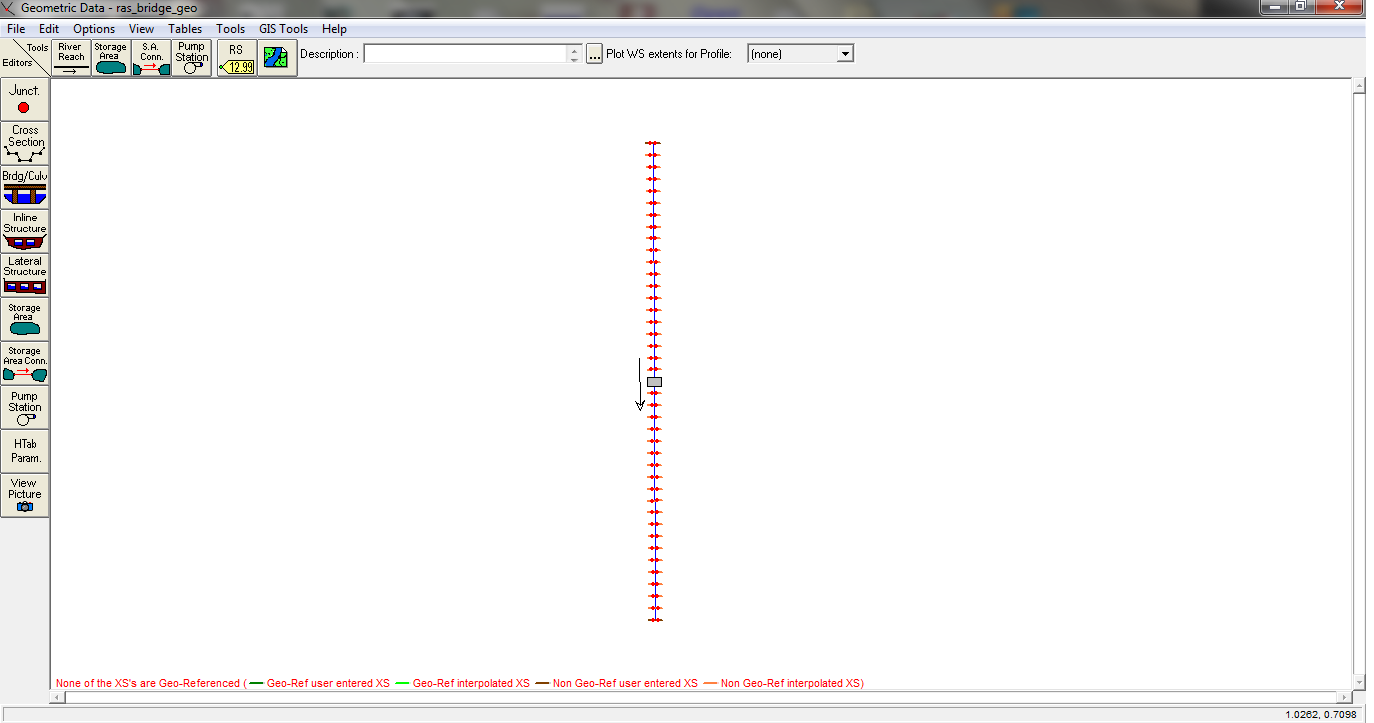
\includegraphics[width=1.0\textwidth]{hecras_bridge_test/RASGeometry_Bridge.png}
\end{center}
\caption{Screenshot showing the HECRAS model geometry schematization}
\label{schematic}
\end{figure}


A discharge timeseries is imposed upstream for both models, with the discharge
increasing from 1m$^3$/s initially to 70m$^3$/s at the end of the simulation.
Details of the model setup can be seen in the code / input files in this
directory.

\subsection{Results}

Figure~\ref{Reach} show stage timeseries at various stations downstream in each model.
The ANUGA and HECRAS results are qualitatively similar. Just upstream of the
bridge (stations 525+), ANUGA shows a backwater effect earlier than HECRAS,
while the final steady-state stage is somewhat lower than in HECRAS. This is
attributable to the different bridge models used (energy equation for HECRAS vs
culvert+shallow-water for ANUGA). HECRAS includes several other bridge models
(based on the momentum equation or other methods), and these would also give
different results. 

\begin{figure}
\begin{center}
\includegraphics[width=0.9\textwidth]{CENTRAL_CHANNEL.png}
\end{center}
\caption{Stage at various points downstream in the channel}
\label{Reach}
\end{figure}

Another minor point is that for the channelised flow, HECRAS computes the
friction slope in the channel using the hydraulic radius, which include the
'bank-drag' effect, whereas ANUGA does not. Hence, even away from the bridge
steady-state results can differ slightly.

